\chapter{Classical Learning Algorithms}
\label{appndx:cla}

\section*{Learning Algorithms}
The goal of a data classification process is to predict an outcome based on some give data. In order to do so, data mining algorithms first process a training set containing a set of attributes and corresponding outcome: a class or a value. Algorithms develop hypotheses that best describe the relationship among the attributes and the outcome for the total instance set.  Formally, learning problems are defined as follows: Given a data set of $m$ instances  $D \equiv \{ \{\vec{x}_1, y_1\}, \{\vec{x}_2, y_2\}, \{\vec{x}_3, y_3\}, \dots, \{\vec{x}_m, y_m\} \}$ where $ \vec{x} = \{x_1, x_2, x_3, \dots, x_n\}$, learning algorithms try to approximate $H \equiv y = f(\vec{x})$. Additional to being typical linear, polynomial, etc. functions, $H$ can also be a set of IF-THEN rules. These rules or functions are then used to predict unseen instances where the outcome class is not known. These algorithms are known as learning algorithms, and in the last few decades, have widely been researched in the field of machine learning. This section briefly discusses a few of the basic algorithms upon which the foundation of ensemble methods and this thesis are laid. The detailed discussion of these algorithms are out of the scope of this chapter. Thus, we discuss only the core concepts here.

\subsection*{$k$-Nearest Neighbors}
The $k$-nearest neighbor algorithm, in short $k$-NN, is one the simplest learning algorithm available. It is a non-parametric instance-based lazy learning algorithm and works for both supervised and unsupervised learning. It uses similarity measures like distance functions to classify unknown instances. The decision is a majority voting of  $k$ neighbors where $k$ is predefined. For example, if $k= 1$ then an unknown instance is assigned the class label of its nearest neighbor. There are several schemes to find the $k$ nearest neighbors. For numeric data, some well-known distance functions are Euclidean distance, Manhattan distance, Minkowski distance, etc.  As in Figure~\ref{fig:bg:knn} the 1-NN classification for the new instance is {--}, 2-NN is undecided or tie, 3-NN is {+} using Euclidean distance.
\begin{itemize}
    \item Euclidean distance $D_E = \sqrt{\sum_{\i =1 }^{k} (x_i - y_i)^2}$
    \item Manhattan distance $D_M = \sum_{\i =1 }^{k} |(x_i - y_i)|$
    \item Minkowski distance $D_{Mink}\sqrt[q]{\sum_{\i =1 }^{k} (|x_i - y_i|)^q}$
\end{itemize}
For categorical data, the Hamming distance can be used. The Hamming distance is defined as $D_H = \sum_{\i =1 }^{k} |(x_i - y_i)|$ where $|x_i - y_i|$ is $0$ if $x=y$, $1$ otherwise.

\begin{figure}[htbp]
    \begin{center}
        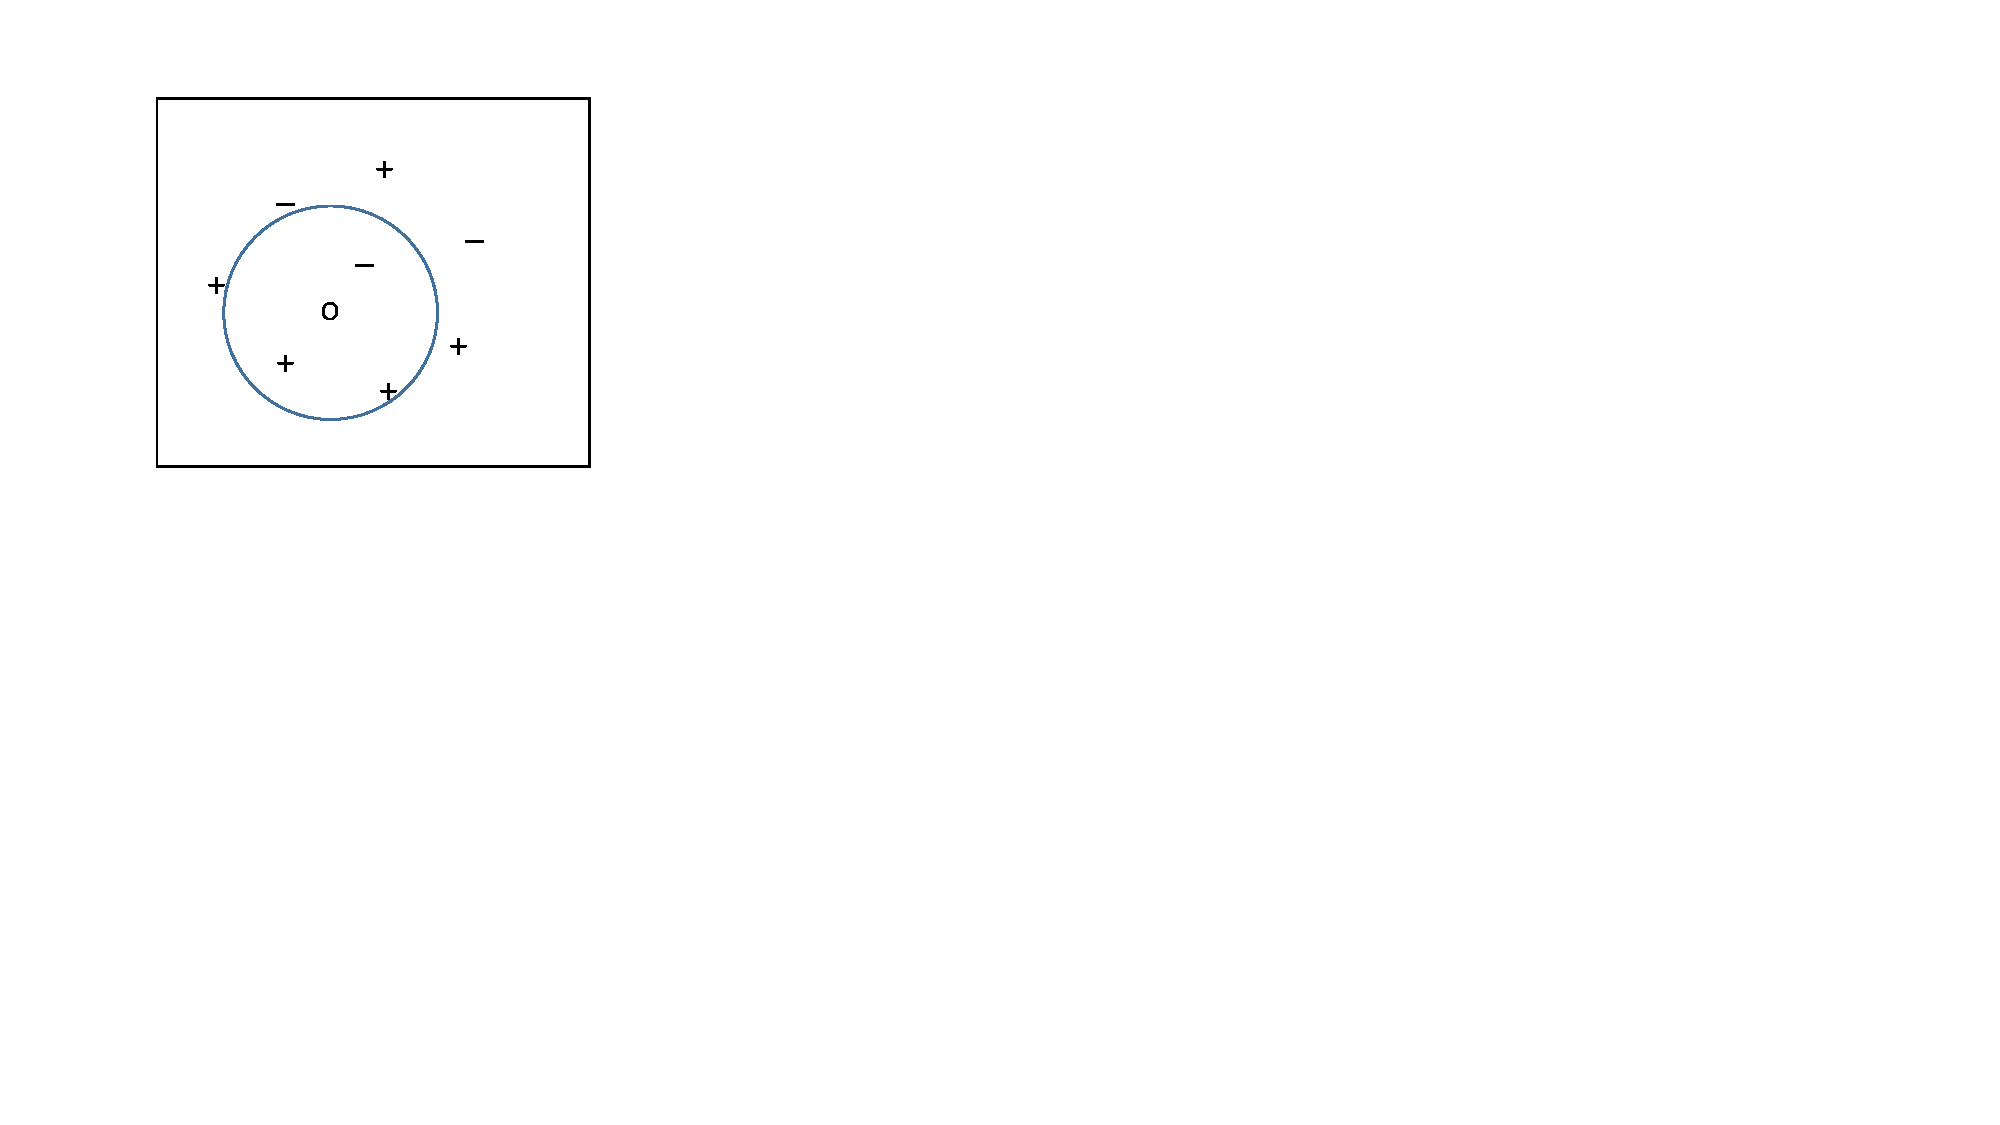
\includegraphics[width=3.0in]{figs/knn.pdf}
        \caption{Concept of $k$-NN classifier}
        \label{fig:bg:knn}
    \end{center}
\end{figure}

Choosing an optimal $k$ is the prime challenge of the $k$-NN algorithm, which is extremely training data dependent. Changing the position of a few training points could lead to a significant loss in performance. The method is particularly not stable in the class boundary. $k$ should be large enough that $k$-NN could overcome the noises in the data, and small enough that instances of other classes are not included. Generally, higher $k$ reduces the overall noise and should be more precise. For most data sets a value between $3$-$10$ performs much better than $1$-NN. Typically, cross-validation is used to determine a good $k$. 

\subsection*{Na\"ive Bayes}
Na\"ive Bayes classification is based on Bayes rule. Bayes rule says that the probability of an event $x$ conditioned on knowing an event $y$, i.e. the probability of $x$ given $y$ is defined as
\[
p(x|y) = \frac{p(x,y)}{p(y)} = \frac{p(y|x) p(x)}{p(y)}
\]
The na\"ive Bayes classifier~\cite{langley92:nb} assumes that all the explanatory variables are independent. Given a feature set $X = x_1, x_2, \dots, x_n$ of $n$ independent variables, na\"ive Bayes assigns the instances to $k$ possible outcomes or classes, $p(C_k | X)$. Using Bayes rule, the conditional probability can be decomposed as:
\[
p(C_k |X) = \frac{p(C_k) p(X|C_k)}{p(X)}.
\]
In other words,
\[
posterior = \frac{prior \times likelihood}{evidence}.
\]
Using the chain rule repetitively, it can be expressed as follows:
\[
p(C_k |X) = p(C_k) \prod_{i=1}^n p(x_i | C_k)
\]
The predicted class is the one which maximizes the conditional probabilities $p(C_k|X)$, that means, the classifier assigns the class label $\hat{y} = C_k$ for some $k$ that satisfies:
\[
\hat{y} = \underset{k \in \{1, \dots, K\}}{argmax}  p(C_k) \prod_{i=1}^n p(x_i | C_k)
\]

\subsection*{Decision Trees}
Decision trees (DTs) are another popular genre of non-parametric supervised learning algorithms. Trees allow a way to graphically organize a sequential decision process. A decision tree, a directed acyclic graph, contains decision nodes, each with branches for all alternate decisions. The leaf nodes are labeled with the respective class label. Each path from the root to the leaf is a decision rule, consisting of a conditional part (unions of all internal nodes' conditions) and a decision (of leaf node).

Decision trees use {\it information gain} to select the splitting attribute that would maximize the total entropy of each of the subtrees resulting from the spit. Entropy is a measurement of purity of an attribute, typically ranged between 0 and 1. A pure attribute, an attribute with a definitive value-class relationship, would have a low entropy and is easy to use for prediction. On the other hand an attribute with a highly mixed value-class relationship would yield high entropy. A common entropy function is:
\[
entropy = - \sum_{i=1}^n p_i \lg p_i.
\]
where $p_1, p_2, \dots, p_n$ are the distributions of several class attributes and $\sum p_i = 1$. The information gain is the difference between old and new entropy after a split. This is a good measurement of relevance of an attribute. However, in cases where an attribute can take on a large number of distinct values, information gain is not ideal. Presence of a large set of values could uniquely identify the classes but also reduces the chance to generalize unseen instances and should be avoided to be placed near root.

A decision tree is, however, computationally feasible. The average cost of constructing a decision tree for $n$ instances with $m$ attributes is $O(mn \lg n)$, and querying time is $O(\lg n)$.

\subsection*{Neural Networks}
The Neural Network (NN) is a learning method inspired by biological neural network. A set of inter-connected nodes (also known as perceptrons and neurons) mimics a biological neural network. Figure~\ref{fig:bg:nnlayer} shows a skeleton of a neural network. A neural network is a weighted directed graph where an input layer is connected to the output layer via some hidden layers. This is commonly known as Multi-Layer Perceptron (MLP). Decisions are made looking only into the output layer only. Hidden layers enlarge the space of hypotheses. If there is no hidden layer, then the  neural network becomes a simple regression problem i.e. output is a linear function of inputs. Each connection among these nodes has an associated weight. Given an input data set, these weights are updated accordingly to best fit the classification model. Learning is done by the back-propagation algorithm~\cite{raul96:nn}. Errors are propagated back from the output layer to the hidden layer and weights are updated to minimize the error.
\begin{figure}[htbp]
    \begin{center}
        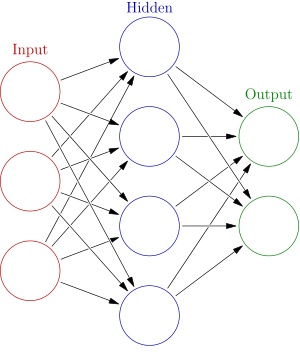
\includegraphics[width=4.0cm]{figs/nnlayers.png}
        \caption{Neural network layers}
        \label{fig:bg:nnlayer}
    \end{center}
\end{figure}

Learning starts with assigning a small value as initial weight to all the connection weights. In case of a single perceptron, the learning process is analogous to moving a parametric hyperplane around. Let $w_i$ be the weight of the $i$-th input, then after $t+1$ iterations the weight $w_i(t+1) = w_i(t) + \nabla E_i(t)$, where $\nabla E_i$ is the gradient of the error function. For an input vector $\mathbf{x}$ and true output $y$, $E$ is defined as the squared error:
\[
E = \frac{1}{2} Err^2 = \frac{1}{2} (y - h_w(\mathbf{x}))^2
\]
Thus gradient of $E$ would be:
\begin{align*}
    \nabla E = \frac{\partial E}{\partial W_j} & = Err \times \frac{\partial Err}{\partial W_j} = Err \times \frac{\partial}{\partial W_j} (y - g(\sum_{j=0}^n w_j x_j)) \\
    & = - Err \times g^{\prime} (in) \times x_j
\end{align*}
Based on this, the weight update rule would be:
\[
w_j = w_j + \alpha \times Err \times g^{\prime} (in) \times x_j
\]
where $\alpha$ is the learning rate coefficient. The back propagation algorithm for multi-layer perceptron also works in similar fashion. Weights in the output layer are updated using the following equation:
\[
w_{j,i} = w_{j,i} + \alpha \times a_j \times \nabla_i
\]
where $\nabla_i = Err \times g^\prime(in_i)$. Hidden layers propagate this error from the output layer using:
\begin{align*}
    \nabla_j &= g^\prime (in_i) \sum_i w_{j,i} \nabla_i \\
    w_{k, j} &= w_{k, j} + \alpha \times a_k \times \nabla_j
\end{align*}

MLP is a very expressive method. Only $1$ hidden layer is sufficient to represent all continuous functions and $2$ can represent any functions. MLP is prone to local minima, which is avoided by running MLP multiple times with different initial weight settings.
\clearpage